\chapter{Superconductivity and quench: an overview}
\label{chp:soupcond-quench}
In this chapter I will explain some of the very basic concepts linked to superconductors and
superconductor quench.
\section{Superconductivity in theory}
\label{sec:soupcond}
Electrical motion in metallic or insulating materials is a very well studied and documented
phenomenon. Electrons passing through any material, endure a varying amount of disturbance in their
motion based on the type and structure of the material, this disturbance is known as resistivity $\rho$.
Given a sample of a material of length $l$ and cross-section $A$ we can compute the resistivity as
shown in \ref{eq:resistivity-cable}
\begin{equation}
	\label{eq:resistivity-cable}
	\rho = \frac{RA}{l} = \frac{m}{ne^2\tau}
\end{equation}
As highlighted in the second part of equation \ref{eq:resistivity-cable}, the resistivity of a
material can be seen as a function of:
\begin{itemize}
	\item The mass of the electron $m$,
	\item The charge density $n$,
	\item The charge of the electron $e$
	\item The relaxation time of the electron, which is the time interval occurring between two
	      successive electronic collisions $\tau$.
\end{itemize}

The resistivity of any material at a certain temperature $\rho_T$ can be written as a function of
the sample's resistivity, at a reference temperature $T_0$, $\rho_0$ and a regularization term
known as the temperature coefficient of resistivity, which is the ratio of resistance change to
temperature change.
\begin{equation}
	\label{eq:resistivity-func-of-temp}
	\rho_T = \rho_0[1 + \alpha(T - T_0)]
\end{equation}

Based on their values of resistivity materials can be divided between metals and insulators. Metals
will have a very low value of resistivity (usually less than $10^{-5}$) while insulators impede the
passing of electric current.
In \cite{slimani2022superconducting} solid band theory is used in conjunction with equation
\ref{eq:resistivity-func-of-temp} to explain the behavior of both metals and insulators in terms of
freedom of movement of the electrons flowing through the crystalline reticle. Increasing the
operation temperature of a sample yields opposite results based on the material: if the sample is a
metal then increasing the operating temperature will provoke an increase in resistivity, if the
sample is an insulator then the resistivity will decrease and, in some cases, the insulator might
start behaving like a metal, favoring the passing of electricity \cite{slimani2022superconducting}.

In 1911 \cite{invention-superconductivity} it was discovered that if a sample of mercury was cooled
until it reached the temperature of $4.2K$ the resistance exerted by the sample on a current travelling
through it fell from a definite real value to $0$, as can be
seen in figure \ref{img:mercury-resistance}, the mercury sample had reached the superconducting state.
\begin{figure}
	\centering
	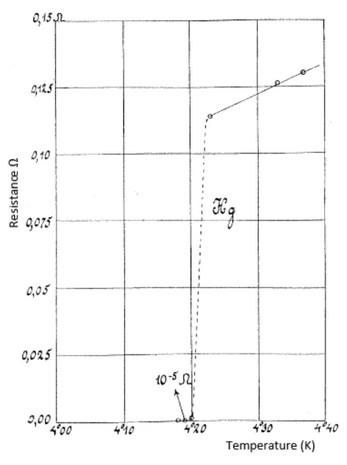
\includegraphics[width=0.5\textwidth]{./img/mercury-resistance.png}
	\caption{The resistance of Mercury in function of the temperature of the sample, taken from
		\cite{tsukerman2020compendium}}
	\label{img:mercury-resistance}
\end{figure}

Later studies discovered that many materials, pure and alloy, could be brought to the
superconducting state as long as three conditions were met:
\begin{itemize}
	\item The temperature of the sample doesn't exceed the critical temperature $\tc$,
	\item The current density passing through the sample doesn't exceed the critical current
	      density $\jc$,
	\item The magnetic field acting on the material doesn't exceed the critical magnetic field $\bc$.
\end{itemize}

When a material reaches the superconducting state it exhibits perfect diamagnetism, which means that
the material is able to perfectly repel magnetic fields, a simple experimental proof of this effect
is given by magnetic levitation. This capacity to repel magnetic fields was first observed by
Meissner and Ochsenfeld in 1933 \cite{meissner1933}. While the repulsion of the magnetic field is
perfect it had already been proven by Geertruida de Haas-Lorentz in 1925 \cite{fokker1925physica}
that magnetic fields do, in fact, penetrate the surface of the superconductor and in 1935 the
original observation was confirmed by the London's equations \cite{london1935}.

The diamagnetic properties of superconductors depend on the strength of the applied magnetic field
and the kind of maerial used for the sample. In general two different types of superconductors have
been found and studied based on their behaviour under the effect of strong magnetic fields.

\section{Type I superconductors}
\label{sec:type1}
As it can be seen in figure \ref{img:type1-transition} Type I superconductors are characterized by a very
sharp fall of their magnetization, which measures the amount of induced or
permanent magnetic dipole moment of a magnet per unit volume \cite{polarization-magnetization}, once
the applied magnetic field reaches $\bc$.
\begin{figure}
	\centering
	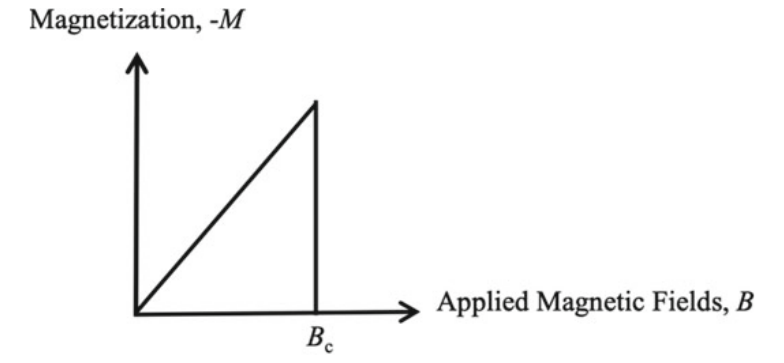
\includegraphics[width=0.75\textwidth]{./img/type1.png}
	\caption{Magnetization of a superconducting coil plotted agains the external magnetic field
		\cite{slimani2022superconducting}}
	\label{img:type1-transition}
\end{figure}
Type I superconductors, as long as the applied magnetic field is less than $\bc$, have diamagnetic
properties, but once the superconductor undergoes a transition to the normal-conducting
state (which will be referred to as \emph{quench} from now on) the magnetic dipole exerted by the
superconductor falls to zero (or a negligible value) allowing magnetic field penetration and making such materials unsuitable for the kind of environments and applications such the ones covered by this thesis.

\section{Type II superconductors}
\label{sec:type2}
Type II superconductors are usually dirtier materials if compared to Type I superconductors, in most
cases the material is an alloy, this characteristical impurity gives Type II superconductors an edge
over Type I due to the magnetization degrading gracefully with the increase of applied magnetic
field. A schema similar to figure \ref{img:type1-transition} can be seen in figure \ref{img:type2-transition}.
\begin{figure}
	\centering
	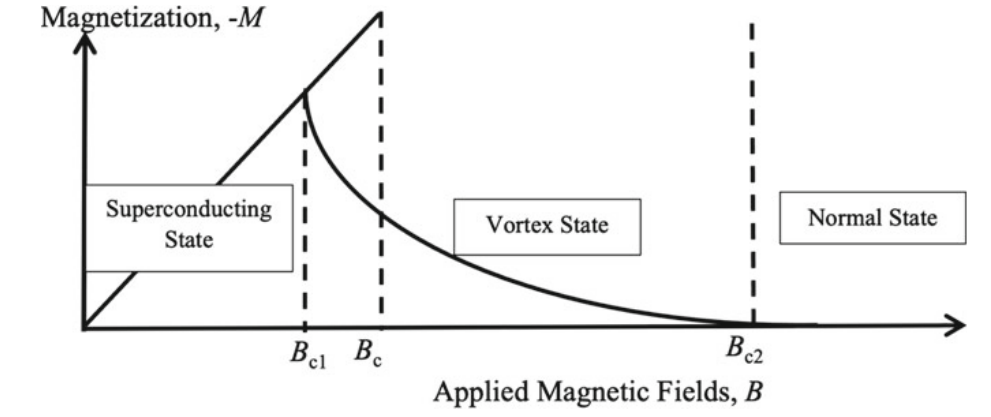
\includegraphics[width=0.75\textwidth]{./img/type2.png}
	\caption{Magnetization of a type II superconducting coil plotted against the external magnetic field
		\cite{slimani2022superconducting}}
	\label{img:type2-transition}
\end{figure}
Type II superconductors, while the applied magnetic field is less than $B_{C1}$ have the same
diamagnetic properties of Type I superconductors but, instead of having a very sharp transition from the superconducting state to
the normal-conducting state once the limit is reached, these materials have an intermediate state referred to as the vortex or hybrid
state.
In the vortex state the external magnetic field is penetrating the surface of the superconductor, but the
flux lines are constrained in particular structures pinned within the reticle of the
superconductor, called Abrikosov vortices or fluxons \cite{abrikosov-vortices}, vortices are constituted of a supercurrent
following a ring trajectory surrounding the magnetic field lines that started penetrating the
material. Since the ring structure is extremely stable \cite{fujita-theory-HTS}, as long as the
fluxons are pinned in place, the material remains
locally superconductive, vortices are usually anchored to imperfections in the material, that is why
(as was said earlier) alloys and dirtier materials are usually Type II superconductors.

Type II superconductors are usually the kind of materials used in applications such as the one
discussed in this thesis due to the high resilience to the influence of external magnetic fields.

\section{Quench}
